\section{Introduction}\label{intro}\sloppy
Recent advances in deep learning have enabled new forms of analysis on images and videos~\cite{lecun2015deep}. 
A typical analytics task is to find all images in a corpus that contain a certain object, e.g., detecting people in CCTV footage, using neural network-based object detection models.  
Deploying such models at scale for visual analytics is a formidable computer systems challenge with significant recent interest from both industry and academia~\cite{kang2017noscope, anderson2018predicate, kang2018blazeit, chetlur2014cudnn, fengeva, zhang2018ffs, anderson2018physical, jiang2018mainstream, jiang2018chameleon}. 
Recent work is increasingly inspired by ideas from relational database systems, where users can specify predicates in a query language and the system uses a neural network to determine which images satisfy those query predicates~\cite{kang2018blazeit,wu2018querying}.
The motivation is that a query language provides the user with a declarative interface that abstracts away low-level implementation and optimization details of the neural network inference.

However, the overarching problem of supporting declarative query answering on the content of videos and images is far from solved.
Consider a simple task: given two videos find a certain object that appears in both videos. For example, we might be interested in determining if the same person appeared in two different CCTV feeds. To answer this query, one has to first find potential target objects in both videos and then match them against each other. There are hidden implementation decisions about indexing (can a multidimensional index be used for faster matching), optimization (if we do index, which video to scan and what type of an index to use), and compression (can the matching be performed on low-dimensional features instead of raw frames). These choices go beyond the intra-operator neural network optimizations seen in~\cite{kang2017noscope, zhang2018ffs, anderson2018physical, jiang2018chameleon}, and are more analogous to physical design and physical operator selection in traditional relational database management systems. In RDBMS, a strong separation of logical and physical concerns enables a declarative user-facing interface and an extensible system-facing interface. In contrast, the data and the query models used in recent video analytics systems lack an analogous separation. The implementations of query filter operators are often tied to specific neural network families, object detection/identification use cases, and data source semantics like ordering.

This paper explores the necessary steps towards a future Visual Data Management System (VDMS).
We built a research prototype system, called \textsf{DeepLens}, where visual analytics tasks are maps, joins, and filters over collections of subimages (called patches) and an associated key-value dictionary storing information about them (e.g., neural net classifications). The query model in \textsf{DeepLens} has set semantics and makes no structural assumptions about the data source, e.g., any timing data in video are stored as additional attributes. Optimizations for performance are introduced through physical design, where \textsf{DeepLens} allows for the materialization, data layout, and both single-attribute and multi-dimensional indexing on patch collections.

\begin{figure}[t]
%\vspace{-5pt}
\centering
 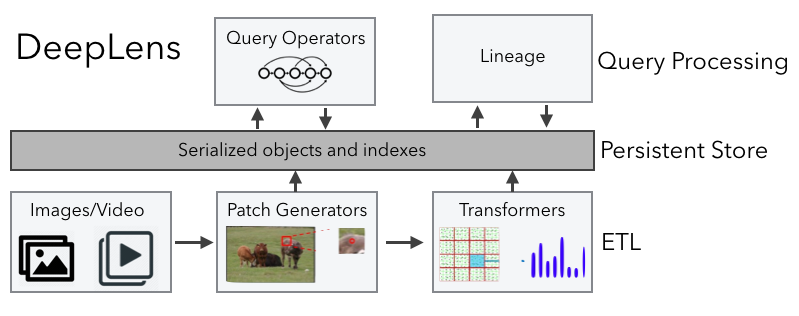
\includegraphics[width=\columnwidth]{figures/teaser.png}
 \caption{DeepLens has a dataflow-like architecture for processing visual analytics queries. All analysis is cast as relational queries on relations of image patches. Intermediate results can be materialized and indexed.  \label{teaser} }
\end{figure}
%\vspace{-5pt}

This architecture disentangles the process that generates the patches (neural network inference in prior work) with the downstream query processing of the collection--similar to the distinction between ETL and query processing in an RDBMS.
The query operators are agnostic to whether those patches represent the output of a neural network, black-box geometric computer vision pipeline, or even the output from crowdsourcing. 
To illustrate the benefits of physical and logical separation, we design a benchmark of six analytics tasks and vary what is indexed, how the operators are implemented, the underlying algorithms, and the properties of the underlying hardware.
 
Simply put, we found that poor design choices can sacrifice multiple orders of magnitude of performance.
\textbf{Indexing: } We found that index usage was crucial and could improve query performance by up-to 612x. However, particularly for the geometric indices, the size and dimensionality of the data plays a key role in how beneficial an index will be.
\textbf{Lineage: }We found that many tasks require relating processed results back to the base data.
Maintaining and indexing tuple-level lineage led to a 60x improvement in one benchmark query.
\textbf{CPU vs. GPU: } Cost-models that accurately balance CPU and GPU utilization for query optimization will be a significant challenge. Some queries benefited by nearly two orders of magnitude, while other actually got slower when processing tasks were offloaded to a GPU.
\textbf{Managing Uncertainty: } Unlike in relational databases, queries in a VDMS are approximate by nature. Traditional optimizations, like filter pushdown, may additionally create different accuracy profiles.  One of our main conclusions is that any future ``declarative'' VDMS will have to \emph{revisit query optimization and automated physical design from a unified perspective of performance and accuracy tradeoffs.}  







